\section{Conclusions}
	\begin{frame}{Author's Conclusions}
		\begin{itemize}
			\item[$\bullet$] Enhancements provided by adiabatic computers for solving \textbf{NP}-Hard or \textbf{NP}-Complete problems
			\item[$\bullet$] Promising result for Quantum Machine Learning
			\item[$\bullet$] The approach targets the global solution of the training problem \textbf{better} than the classic alternatives
			\item[$\bullet$] The \textbf{D-Wave 2000Q} machine
			\item[$\bullet$] Quantum approach partitions data with similar accuracy to the classical approaches
			\item[$\bullet$] The approach assumes viability as the quantum hardware improves
		\end{itemize}
	\end{frame}
	% First conclusion is related to the possibility of quantum annealers to solve efficiently optimization problems belonging to the NP-Hard and NP-Complete classes
	% Hence, being machine learning mainly focused on solving optimization problems we have very promising results for the field of Quantum Machine Learning
	% Results are similar to the ones that we obtained with the classical algorithms. Experiments were run testing different scalability parameters and in all we were able to understand that quantum hardware is always the main limitation. What it is expected with the development of the technology is that the quantum solver will be able to outperfrom the classical ones and also solve more complex instances of problems

	% REMIND that everything was tested on the 2000q machine and nowadays we have a machine that is more powerull -> Advantage (start to introduce the importance of our last critic)

	\begin{frame}{Future Works}
		\small{
		\begin{itemize}
			\setlength\itemsep{-0.5em}
			\item[$\bullet$] Bring the QUBO formulation to the generic k-means training problem
				\begin{itemize}
					\setlength\itemsep{-0.5em}
					\item[$\circ$] \textbf{Balanced Problem} \small{$$\min _{\Phi} \sum_{j=1}^{k} \frac{1}{2\left|\phi_{j}\right|} \sum_{x, y \in \phi_{j}}\|x-y\|^{2} \implies \min _{\Phi} \sum_{j=1}^{k} \sum_{x, y \in \phi_{j}}\|x-y\|^{2}$$}
					\item[$\circ$] \textbf{Generic Problem} \small{$$\min _{\Phi} \sum_{j=1}^{k} \frac{1}{2\left|\phi_{j}\right|} \sum_{x, y \in \phi_{j}}\|x-y\|^{2}$$}
				\end{itemize}
			\item[$\bullet$] Use elements of the approach to formulate quantum algorithms for similar clustering models
			\begin{itemize}
				\item[$\circ$] k-medoids clustering
				\item[$\circ$] fuzzy C-means clustering
			\end{itemize}
			\item[$\bullet$] Cluster larger datasets 
		\end{itemize}
		}
	\end{frame}
	% Future works are mainly based on working on the QUBO formulation
	% In fact an interesting development could be the one of generalizing the formulation to the generic k-means training problem. We tried to understand what this work would require. Trivial is to remove the constraints that we added for the balanced problem but in this way the formulation gets different and the step that follow in the procedure of obtaining the final formulation may be more complex than the ones that Matteo presented. An example is what happens on |phi_j|: thanks to the balanced assumption we are allowed to remove the term while in the generic case we should bring the complete formulation to a suitable QUBO. We have to be careful in the discussion on the tuning of parameter alpha since allowing the problem to be more unbalanced is still assuming that the term |phi_j| has been removed.

	% Using the QUBO formulation the authors say that they could also think of formalizing similar clustering models to solve other instances of such problem like: k-medoids and fuzzy C-means
	% The main and more interesting work that we all can't wait to discover is whether the promises made by the authors are valid when we consider larger datasets

\section{Critical View}
	\begin{frame}[allowframebreaks]{Critical View}
		\textbf{How complex is to construct the QUBO ?}
		$$\min _{\Phi} \sum_{j=1}^{k} \sum_{x, y \in \phi_{j}}\|x-y\|^{2}$$ $$\big\Downarrow$$ $$\min _{\hat{w}} \hat{w}^{T}\left(I_{k} \otimes(D+\alpha F)+Q^{T}\left(I_{N} \otimes \beta G\right) Q\right) \hat{w}$$ 
		
		\textbf{Complexity}: $O(N^2kd)$ \\
		Since $kd < N$:
		\begin{itemize}
			\item[$\bullet$] \textbf{Better} than classical balanced k-means: $O(N^3)$
			\item[$\bullet$] \textbf{Worse} than Scikit Learn implementation: $O(Nkd)$  
		\end{itemize}
		% Our critical view on this paper is mainly focused on the study of the QUBO formulation since we think that this step, in each of the quantum annealing papers describing how to solve a problem in this way, is the most important. This because if we are able to bring the classical optimization problem to the QUBO formulation, more than limitations regarding the hardware of the quantum machine, we are already able to write an algorithm that can be executed on the annealer.
		% For this reason the first conclusion that we want to address is understanding how complex is to construct the QUBO. To answer this question it means to understand the complexity needed to pass from the equation on the top (the formal classical balanced k-means opt problem) to the one on the bottom (the final QUBO formulation). As we were able to understand from Matteo's description of the QUBO formulation the terms in this equation determine a complexity of O(N^2kd). Since kd < N it means that in general the quantum algorithm performs better than classical balanced k-means O(N^3) and worse than Scikit Learn O(Nkd).
		
		\framebreak
		\small{
		Hyperparameter $\alpha$ allows to make considerations in the data preparation phase of the clustering algorithm:
		\begin{itemize}
			\item[$\bullet$] \textbf{Completely unbalanced} $\implies$ use Scikit-Learn implementation
			\item[$\bullet$] \textbf{Fairly Balanced} $\implies$ tuning on $\alpha$ and use Quantum Balanced implementation
			\item[$\bullet$] \textbf{Balanced} $\implies$ use Quantum Balanced implementation with $\alpha < \beta$
		\end{itemize}
		\textbf{Tuning $\alpha$}
		\begin{itemize}
			\item[$\bullet$] Modifies the curvature of the quadratic function to optimize
			\item[$\bullet$] By making $\alpha$ looser we change the position of the optimum allowing to cluster datasets that are not completely balanced
			\item[$\bullet$] Tuning $\alpha$ allows to prepare the algorithm on how much balanced the dataset will be 
		\end{itemize}
		}
		% The parameter alpha determines the possibility of allowing to violate the constraint of having unbalanced classes. Remember however that our QUBO formulation is based on the assumptions that clusters have the same size, this is a consequence of removing |phi_j| from the formulation. For this reason, this discussion works well for clustering problems that are almost balanced. This is obvious if we concentrate on what the 3 algorithms that we are studying are made for. Scikit-Learn implementation solves the general problem, hence it is obvious that for a generic problem, choosing this rather than the quantum balanced algorithm will perform better. The opposite happens for a balanced problem, but in this case we also have to face the complexity related to the technology on which we are running our quantum algorithm. What we want to study, tuning alpha is in the middle between these opposites. Matteo showed how alpha is used to loose the constraint on the balancing of the classes: choosing a looser value will allow us to violate the constraint even more. However always remember on the assumption that we made on |phi_j|
		% Tuning alpha modifies the curvature of the quadratic problem to optimize. Hence if the optimum of the balanced formulation is moved upwards thanks to a looser alpha, it means that we are allowing for the constraint to be violated more. In this way we will be able to find a solution for the case when more points belong to a class with respect to the others. Obviously this works in the case that we know that the dataset that we are going to consider has this characteristic. In the general case setting alpha smaller than beta is the best practice, always to allow the possibility to violate a few the constraint
	
		\framebreak
		\textbf{Variables and Embedding of the QUBO}
		\begin{itemize}
			\item[$\bullet$] In the QUBO formulation we introduce $k$ binary variables for each variable in the original problem \\ $$O(Nk) \:\: \textbf{variables}$$ % complexity of equation above [16]
			\item[$\bullet$] Efficient embedding algorithms \textcolor{gray}{[30]} allow for a density of \\ $$O(N^2 k^2) \:\: \textbf{qubits}$$ 
		\end{itemize}
		\vspace{-0.5cm}
		\begin{figure}
			\centering
			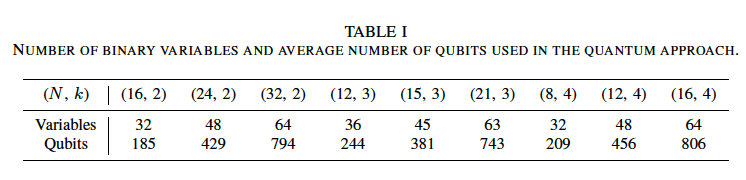
\includegraphics[scale=0.7]{table1.png}
		\end{figure}
		\vspace{-0.3cm}
		\tiny{\textcolor{gray}{[30] P. Date, R. Patton, C. Schuman, and T. Potok, “Efficiently embedding qubo problems on adiabatic quantum computers,” Quantum Information Processing, vol. 18, no. 4, p. 117, 2019.}}
		% The second consideration related to the qubo formulation is its density and consequently the number of qubits that the problem needs to be embedded on the quantum annealer. As we clearly understood from Matteo's discussion since k binary variables are needed for each of the N points we will have Nk variables in the final problem.
		% Now the problem needs to be embedded on the quantum annealer and, even  by using the most efficient annealing algorithms this process requires a quadratic time and a quadratic footprint of qubits. This means that the complexity of the number of qubits that are required to embed the problem is O(N^2k^2)

		% It is interesting to compare this complexity to the table reported by the authors for their experiments. From the table we can see that the relation between the variables and the qubits is still not quadratic. The reason of this is because we are considering problems that are still too simple. For small values it is clear in a relation like 0.0000001x^2 + 0.01x + 0.0001c that the linear and constant term are the ones dominating, while if we increase the size what we will observe is the quadratic upper bound.
		
		\framebreak
		\normalsize
		\textbf{Can we cluster larger datasets on Advantage?}
		\begin{center}
			\begin{minipage}{0.5\textwidth}
				D-Wave 2000Q
				\begin{itemize}
					\item[$\bullet$] 2048 qubits
					\item[$\bullet$] 6,016 couplers
					\item[$\bullet$] 128,472 JJs
				\end{itemize}
				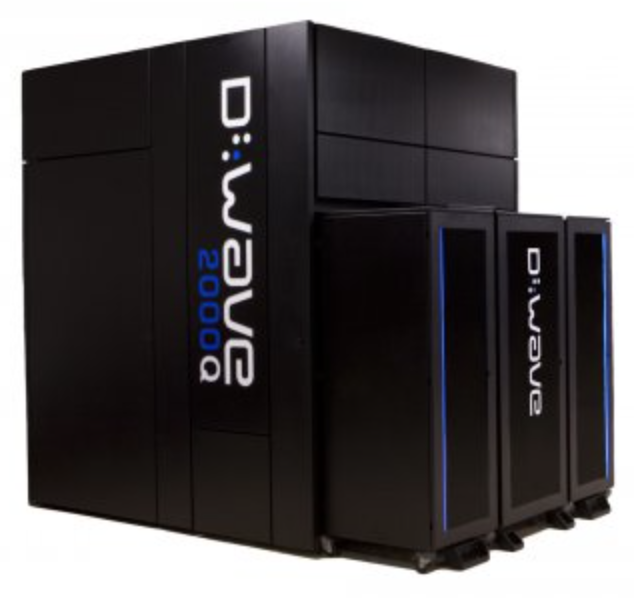
\includegraphics[scale=0.3]{2000Q.png}
			\end{minipage}~
			\begin{minipage}{0.5\textwidth}
				Advantage
				\begin{itemize}
					\item[$\bullet$] 5640 qubits
					\item[$\bullet$] 40,484 couplers
					\item[$\bullet$] 1,030,000 JJs
				\end{itemize}
				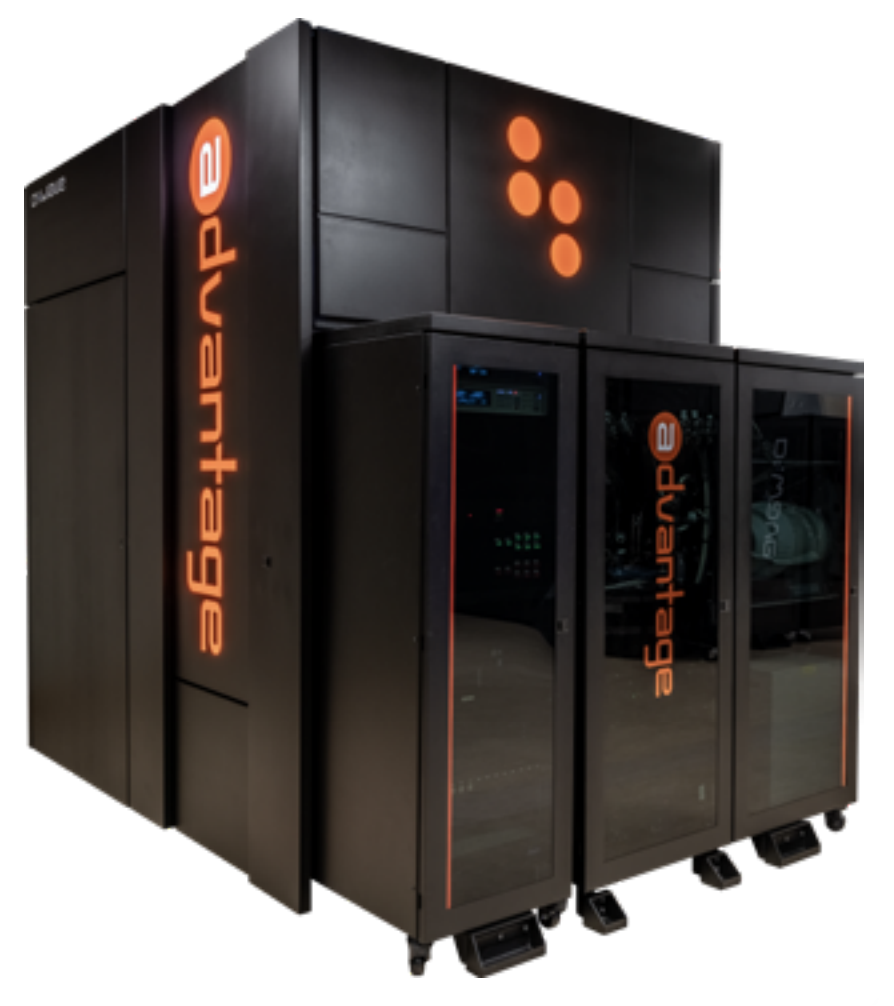
\includegraphics[scale=0.2]{Advantage.png}
			\end{minipage}
		\end{center}
		% Our last conclusion is related to the main topic that we discussed in this paper: technology limitations do not allow to obtain results for complex instances of problems. For this reason we noticed that when the authors were developing this paper the 2000q machine was the only one available. Nowadays we have Advantage, and as we can see in the comparison a big improvement was achieved with this new hardware: more than the double of the qubits and 40k couplers. This conclusion wants to highlight the fact that if the promises of the authors were correct it would be very interesting to check if by using advantage we can already see some better results!
	\end{frame}